\section{Syntax of \lang{}}
\label{sec:syntax}

In this section, we introduce the syntax of \lang{}. A \lang{} program, as shown in the following block, essentially contains several parts,
\begin{bnf}
    \ntsym{program} ::=  (& \ntsym{typedef} | \ntsym{function} | \ntsym{automaton} | \ntsym{system})^*
\end{bnf}

% TODO: make it clear
\begin{enumerate}
    \item \emph{Typedef}s that give aliases to specified types.
    \item \emph{Function} definitions that defines customized functions.
    \item \emph{Automaton} blocks that describe an automaton with given parameters.
    \item \emph{System} blocks to compose automata as components or connections.
\end{enumerate}

\subsection{Type System}
\label{subsec:typesystem}
\lang{} provides a rich-featured type system that supports various commonly-used data types in both formal modeling languages and programming languages.

\smalltitle{Primitive Types} Table. \ref{table:primitivetypes} shows the primitive types supported in \lang{}.

\begin{table}
    \caption{Primitive Data Types}
    \label{table:primitivetypes}
    \centering
    \begin{tabular}{lcr}
        \hline
        Name & Declaration & Term Example \T\B \\
        \hline
        \T Bounded Integer\hspace{0.5cm} & \texttt{int lowerBound .. upperBound}\hspace{0.5cm} & \texttt{-1,0,1} \\
        Integer & \texttt{int} & \texttt{-1,0,1} \\
        Real & \texttt{real} & \texttt{0.1, 1E-3} \\
        Boolean & \texttt{bool} & \texttt{true, false} \\
        Character & \texttt{char} & \texttt{'a', 'b'} \\
        \B Enumeration & \texttt{enum {item$_1$, ..., item$_n$}} & \texttt{enumname.item} \\
        \hline
    \end{tabular}
\end{table}

\noindent\emph{Composite Types.} Composite types offer an approach to contruct complex data types with simpler ones. Several composite patterns are introduced as follows,

\begin{table}
    \caption{Composite Data Types (\texttt{T} denotes an arbitrary data type)}
    \centering
    \begin{tabular}{lr}
        \hline
        Name & Declaration \T\B \\
        \hline
        \T Tuple  & \texttt{T$_1$,...,T$_n$ }\\
        Union & \texttt{T$_1$|...|T$_n$ } \\
        Array & \texttt{T [length]}\\
        Slice & \texttt{T []} \\
        Map & \texttt{map [T$_{key}$] T$_{value}$} \\
        Struct\hspace{1cm} & \texttt{struct \{ field$_1$:T$_1$,..., field$_n$:T$_n$ \}} \\
        \B Initialized & \texttt{T$_{base}$ init term} \\
        \hline
    \end{tabular}
\end{table}

\begin{itemize}
    \item \emph{Tuple}. The \emph{tuple} operator `,' can be used to construct a finite tuple type with several base types.
    \item \emph{Union}. The \emph{union} operator `$|$' is designed to combine \emph{disjoint} types as a more complicated one. This is similar to the union type in C language but much easier to use.
    \item \emph{Array} and \emph{Slice}. An \emph{array} $T[n]$ is a finite ordered collection containing exactly $n$ elements of type $T$. Moreover, a \emph{slice} is an array of which the capacity is not specified, i.e. slice is a dynamic array.
    \item \emph{Map}. A \emph{map }[$T_{key}$] $T_{val}$ is a dictionary that maps a key of type $T_{key}$ to a value of type $T_{val}$.
    \item \emph{Struct}. A \emph{struct }\{$field_1:T_1,\cdots,field_n:T_n$\} contain $n$ fields, each has a particular type $T_i$ and a unique identifier $id_i$.
    \item \emph{Initialized}. A initialized type make it able to specify default values to types.
\end{itemize}

For simplicity in formalizing data types, we introduce the concept \emph{domain} of a type. 

\begin{formalization}[Domain]
    We use $Dom(T)$ to denote the value domain of type $T$, i.e. the set of all possible value of $T$.
\end{formalization}

\begin{example}[Types Used in A Queue] Now let us introduce some type declarations and local variables used in an automaton \texttt{Queue}. As shown in the following code fragment, we declares a singleton enumeration \texttt{NULL}, which contains only one element \texttt{null}. The buffer of a queue is in turn formalized as an array of \texttt{T} or \texttt{NULL}, indicating that a queue element can be either an assigned item or empty. The head and tail pointer are defined as two bounded integers.
\begin{lstlisting}
typedef enum {null} init null as NULL;
automaton <T:type,size:int> Queue(A:in T, B:out T) {
    variables {
        buf : ((T | NULL) init null) [size];
        phead : int 0 .. (size - 1) init 0;
        ptail : int 0 .. (size - 1) init 0;
    }
    ...
}
\end{lstlisting}
\label{exp:typeinqueue}
\end{example}

\noindent\emph{Parameter Types}. On many occasions, you may want to define a generalizable structure that includes a template function or template component. For example, a binary operator that support various operation ($+$,$\times$, etc.), or an encrypted communication system that can make use of different encryption components. Parameter types make it able to take functions and components (or systems, of course) as a template parameter. But such types will be resolved in instantiation, and hence can only be used in templates of instantiable structures (automata and systems). 
\begin{enumerate}
    \item \emph{An Interface}, denoted by \texttt{interface (port$_1$:T$_1$,$\cdots,$port$_n$:T$_n$)}, defines a parameter that could be any \emph{automaton} or \emph{system} that have exactly the same interface (i.e. both number and directions of the ports are matching). Interfaces are only used in templates of \emph{system}s.
    \item \emph{A Function}, denoted by \texttt{func (arg$_1$:T$_1$,$\cdots, $arg$_n$:T$_n$) : T}, defines a function that have the same argument types and return types. Functions are permitted to show up in templates of \emph{system}s and \emph{automata}.
\end{enumerate}
In Example. \ref{exp:clustersystem} we have a system with a \emph{interface} parameter.

\subsection{Functions}
Functions make it able to encapsulate complex computations and reuse them. In \lang{}, the functions are a bit different from common programming languages -- they include no control statements but assignments. This design makes functions' behavior more predictable (i.e. it can be simplified into a single mathematical representation). For the same reason, functions have access only to its local variables and arguments.

The abstract syntax tree of functions is shown as follows.

\begin{bnf}
    \ntsym{funcDecl} ::= & \tsym{function} \ntsym{template}^? \ntsym{identifier} \tsym{(} \ntsym{arguments} \tsym{)} \tsym{\{} \\
    & (\tsym{variables} \tsym{\{} \ntsym{varDecl}^* \tsym{\}})^? \\
    & \tsym{statements} \tsym{\{} \ntsym{assignStmt}^* \ntsym{returnStmt} \tsym{\}} \\
    \ntsym{assignStmt} ::= & \ntsym{term} \tsym{:=} \ntsym{term} \\
    \ntsym{returnStmt} ::= & \tsym{return} \ntsym{term} \\
    \ntsym{varDecl} ::= & \ntsym{identifier} \tsym{:} \ntsym{type} (\tsym{init} \ntsym{term})^? 
\end{bnf}

Basically, definition of a function includes the following parts.

\smalltitle{Template} A function may contains an optional template including a set of parameters. A parameter can be either a \emph{type} parameter (decorated by \texttt{type}) or a \emph{value} parameter (decorated by its type). Values of the parameters should be determined in compiling-time. Once a parameter is declared, it can be referenced in all the following language elements, e.g. \emph{a) the following parameter declarations}, \emph{b) arguments and return types} and \emph{c) function statements.}

\smalltitle{Name} An identifier that indicates the name of this function.

\smalltitle{Type} Type of a function (\texttt{func} type in Section. \ref{subsec:typesystem}) is determined by its \emph{a) number of arguments, b) type of arguments and c) type of return value.} Note that here the arguments are read-only. In other words, any assignment to an argument is strictly prohibited.

\smalltitle{Body} Body of a function includes an optional set of local variables and a list of ordered statements that describes how the return value is calculated. It must be ended by a \texttt{return} statement.


\begin{example}[Incline Operation on Bounded Integers] Incline operation of pointers are commonly used in a \emph{round-robin} queue, where storage are reused circularly. The \texttt{next} function shows that how pointers in such queues (denoted by a bounded integer) incline. 
    \label{exp:successor_function}
    \begin{lstlisting}
function <size:int> next(pcurr:int 0..(size-1)) : int 0..(size-1) {
    statements { return (pcurr + 1) % size; }
}
    \end{lstlisting}
\end{example}

% TODO: a more complicated function

\subsection{Automaton : The Basic Behavioral Unit}

\begin{bnf}
    \ntsym{automaton} ::=& \tsym{automaton}\ntsym{template}^?\ntsym{identifier} \tsym{(} \ntsym{port}^* \tsym{)} \tsym{\{}\\
    & (\tsym{variables} \tsym{\{} \ntsym{varDecl}^* \tsym{\}})^? \\
    & \tsym{transitions} \tsym{\{} \ntsym{transition}^* \tsym{\}} \tsym{\}} \\
    \ntsym{port} ::=& \ntsym{identifier} \tsym{:} (\tsym{in}|\tsym{out}) \ntsym{type} \\
    \ntsym{transition} ::=& \ntsym{guardedStmt} | \tsym{group} \tsym{\{} \ntsym{guardedStmt}^* \tsym{\}}\\
    \ntsym{guardedStmt} ::=& \ntsym{term} \tsym{->} (\ntsym{stmt} | \tsym{\{} \ntsym{stmt}^* \tsym{\}}) \\
    \ntsym{stmt} ::=& \ntsym{term} \tsym{:=} \ntsym{term} | \tsym{sync} \ntsym{identifier}^+
\end{bnf}

\smalltitle{Template} Compared with templates in functions, template in an automaton supports parameters of \emph{function type}.

\smalltitle{Name} The identifier of automaton.

\smalltitle{Type} Type of an automaton (an \texttt{interface} type in Section \ref{subsec:typesystem}) is determined by the \emph{number} and \emph{type}s of its ports. Type of a port in an automaton contains a prefix, either \texttt{in} or \texttt{out}, indicating the direction of its data-flow, and a normal data type as a suffix. To ensure the well-defineness of automata, ports are required to have an \emph{initialized} type, e.g. \texttt{int 0..1 init 0} instead of \sout{\texttt{int 0..1}}.

\smalltitle{Variables} Two types of variables are used in a automaton definition, they are:
\begin{enumerate}
    \item \emph{Local variables} that are declared in the \emph{variables} section. 
    \item \emph{Adjoint variables} used to describe the status of ports. Syntactically, they are denoted as built-in fields of ports. For example, considering a port A, we assume that it has two boolean fields \texttt{A.reqRead} and \texttt{A.reqWrite} indicating if there is a pending \emph{read} or \emph{write} request on this port, and a data field \texttt{A.value} indicating the current value of this port.
\end{enumerate}

We require that for an output port the \texttt{reqRead} field is read-only and the \texttt{reqWrite} field is writable. Similarly, for an input port the \texttt{reqRead} field is writable but its \texttt{reqWrite} field is read-only. The \texttt{value} field can be overwritten only in an output port.

\smalltitle{Transitions}
In \lang{}, behavior of a automaton is described by a set of guarded transitions (groups), with no explicit concept of locations. As shown in  Example \ref{exp:trans_queue}, a \emph{transition} (denoted by \emph{guard} \texttt{->} \emph{statements}) comprises two parts, a boolean term \emph{guard} that declares the activating condition of this transition, and a (set of) statement(s) that describe how the variables are updated when the transition is fired.

Currently, we have two types of statements supported in automata, they are:
\begin{itemize}
    \item \emph{Assignment Statement} (\texttt{var$_1$,...,var$_n$ := term$_1$,...,term$_n$}). An assignment statement supports multiple assignments at the same time, where local variables and writable adjoint variables are permitted to be assigned.
    \item \emph{Synchronizing Statement} (\texttt{sync port$_1$,...,port$_n$}). Synchronizing statements are synchronizing \emph{flag}s used when joining multiple automata. More details about synchronizing statements are introduced in Section \ref{subsec:composition}.
\end{itemize}

With the introduction of shared variables, synchronizing transitions in automata joining is not as easy as in traditional automata where all variables are local. Informally speaking, the synchronizing statements are used to create a proper schedule of assignment statements so that assignments of shared variables are performed before referring them.

Synchronizing statements are also important flags to distinguish external transitions and internal transitions. A transition is called \emph{external} iff. it synchronizes with its environment through some ports, or \emph{internal} otherwise. Literally, all transitions, where synchronizing statements are involved, are \emph{external} transitions. In such transitions, the following rules are strictly required to avoid read/write conflicts.

\begin{enumerate}
    \item Any assignment statements including reference to an input port (A, for example) should be placed after its corresponding synchronizing statement \texttt{sync A}.
    \item Any assignment statements to an output port (B, for example) should be placed before its corresponding synchronizing statement \texttt{sync B}.
\end{enumerate}

\begin{formalization}[Transitions]
Formally, we use $g\rightarrow S$ to denote a transition, where $g$ is the guard formula and $S=\{s_1,\cdots,s_n\}$ is a set of statements. 
\end{formalization}
Different from a typical automaton, transitions in \lang{} automata are organized with \emph{priority}. A transition has higher priority iff. it is placed in front of the other one. And when multiple transitions are activated by the environment, the one with highest priority will be fired first. For example, suppose $g_1\rightarrow S_1,\cdots,g_n\rightarrow S_n$ is a list of transitions, we could use an equivalent form to rewrite them as the followings, where priority is not required any more.
\[
    g_1\rightarrow S_1, \lnot g_1\land g_2\rightarrow S_2,\cdots,\lnot g_1\land \lnot g_2\land\cdots\land \lnot g_{n-1} \land g_n\rightarrow S_n
\]

\begin{example}[Transitions in Queue] In a queue, we use internal transitions to capture the changes of environment and perform corresponding updates consistently. For example, the input port $A$ (already defined in Example. \ref{exp:typeinqueue}) becomes ready to read (i.e. \texttt{reqRead} set to \emph{true}) when the buffer is not full, and the output port $B$ becomes ready to write when the buffer is not empty, and vice versa. External transitions, on the other hand, mainly show the details of the enqueue and dequeue operations.
\begin{lstlisting}
// internal transitions
B.reqWrite && (buf[ptail] == null) -> B.reqWrite := false;
!B.reqWrite && (buf[ptail] != null) -> B.reqWrite := true;
A.reqRead && (buf[phead] != null) -> B.reqRead := false;
!A.reqRead && (buf[phead] == null) -> B.reqRead := true;

// enqueue operation (as an external transition)
(A.reqRead && A.reqWrite) -> {
    sync A; buf[phead] := A.value; phead := next(phead);
}
// dequeue operation (as an external transition)
(B.reqRead && B.reqWrite) -> {
    B.value := buf[ptail]; ptail := next(ptail); sync B;
}
\end{lstlisting}
\label{exp:trans_queue}
% TODO: explain the transitions
\end{example}

Priority of transitions make the automaton fully deterministic. However, in some cases non-determinism is still more than necessary. \emph{Transition groups} are, consequently, imported to handle such cases. When encapsulated by a group, transitions are unordered and don't ruled by priority. Instead, the group itself is literally ordered w.r.t. other groups and single transitions (basically we can take all single transitions as a trivial transition group).

\begin{formalization}[Transition Groups]
    A transition group $t_G$ is formalized as a finite list of guarded transitions
    \[
        t_G=\{t_1,\cdots, t_n\}, t_i=g_i\rightarrow S_i
    \]
    where $t_i$ is a single transition with guard $g_i$ and a set of statements $S_i$.
    \label{fmz:tgroup}
\end{formalization}

Since a single transition $g\rightarrow S$ can be equivalently written as a singleton group $\{g\rightarrow S\}$, it's acceptable if we assume that each automaton comprises a set of transition groups but no standalone transitions.

\begin{example}[Yet Another Queue Implementation] Let's consider the external transitions in Example. \ref{exp:trans_queue} which captures the core behavior of a queue. When both enqueue and dequeue operations are activated, in that example, reading will always be fired first. Such a queue may get stuff up immediately when requests start accumulating. But here we presents another non-deterministic implementation based on \emph{transition groups} to solve this problem.
\begin{lstlisting}
group {
    // enqueue operation (as an external transition)
    (A.reqRead && A.reqWrite) -> {
        sync A; buf[phead] := A.value; phead := next(phead);
    }
    // dequeue operation (as an external transition)
    (B.reqRead && B.reqWrite) -> {
        B.value := buf[ptail]; ptail := next(ptail); sync B;
    }
}
\end{lstlisting}
In this code fragment above, the two transitions are encapsulated in a group. Consequently, firing of the dequeue operation doesn't rely on deactivation of the enqueue operation.
\label{exp:transgroup_queue}
\end{example}

With all the language elements of an automaton properly formalized, now we introduced the formalization of a complete automaton.

\begin{formalization}[Automata]
    \label{fmz:automata}
    We use a tuple $A=\langle Ports, Vars, Trans_G \rangle$ to represent an automaton, where $Ports$ is a set of ports, $Vars$ is a set of local variables and $Trans_G=\{t_{G_1},\cdots,t_{G_n}\}$ is a set of transition groups that are defines in Formalization. \ref{fmz:tgroup}.
\end{formalization}

\subsection{System : The Composition Approach}
\label{subsec:system}

Theoretically, an automaton in \lang{} is powerful enough to represent any classical software system (where time and probability are not involved, of course). However, modeling complex systems through a mess of transitions and tons of local variables may become a real disaster.

As we have mentioned previously, \lang{} is designed to help the programmers, even nonprofessionals, to enjoy the convenience of formal tools. To achieve this goal, we introduce a new language element called \emph{system}. Basically, a \emph{system} is a textural format of a hierarchical diagram (see in Figure. \ref{fig:diagram}) where automata and smaller systems are naturally organized as different roles (\emph{component}s or 
\emph{connection}s). Both \emph{components} and \emph{connectors} (or \emph{channels}) are well-known concepts in component-based software engineering. Though having different names, their semantics all turn out to the same nature, \emph{automata}.

Hierarchical diagrams have already been used in various modeling tools (for example, SCADE\cite{AbdullaISoLA2006,BerryScp1992}, Simulink and LabVIEW) and formal languages (Reo\cite{ArbabMscsReo2004}, AADL). However, in most tools, connections are simply synchronous link that seal two ports together. Inspired by Reo, we make it able to declare an automaton as a connection, which lead to more powerful and intuitive diagrams. 

\begin{example}[Hierarchical Diagram of a Middleware]
    Figure. \ref{fig:diagram} gives a simple diagram of a message-oriented middleware, where a queue work as a connector to coordinate between the components (message producers and consumers).
\end{example}

\begin{figure}
    \centering
    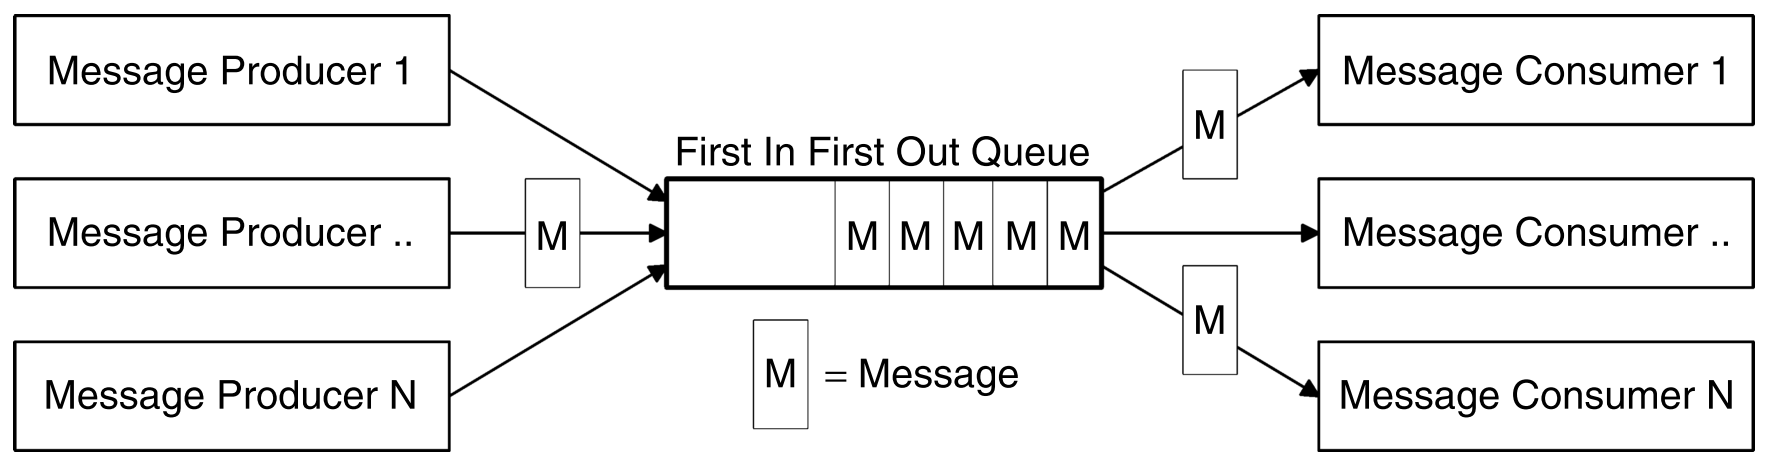
\includegraphics[width=.8\textwidth]{images/middleware_queue.png}
    \caption{A Senerio where Queue is used in Message-Oriented Middleware\cite{CurryMfc2004}}
    \label{fig:diagram}
\end{figure}

The abstract syntax tree of \emph{system}s is shown as follows.
\begin{bnf}
    \ntsym{system} ::= & \tsym{system} \ntsym{template}^?\ntsym{identifier} \tsym{(} \ntsym{port}^* \tsym{)} \tsym{\{}\\
    & (\tsym{internals} \ntsym{identifier}^+)^? \\
    & (\tsym{components} \tsym{\{} \ntsym{componentDecl}^* \tsym{\}})^? \\
    & \tsym{connections} \tsym{\{} \ntsym{connectionDecl}^* \tsym{\}} \tsym{\}}\\
    \ntsym{componentDecl} ::= & \ntsym{identifier}^+ \tsym{:} \ntsym{systemType} \\
    \ntsym{connectionDecl} ::= & \ntsym{systemType} \ntsym{params} \tsym{(} \ntsym{portName}^+ \tsym{)}
\end{bnf}

The \emph{type} of a system (i.e. its template, name, and ports) shares exactly the same form and meaning with \emph{type} of an automaton. This also suggests that system is NOT a special semantics unit, but simply an compositional approach to pile up automata. We declare a system with its template, name and type, then it is implemented by an optional set of \emph{internal node}s, an optional set of \emph{component}s and a set of \emph{connection}s.

\smalltitle{Template} In templates of systems, all parameters types are supported including \emph{a)} parameters of abstract type \texttt{type}, \emph{b)} parameters of primitive types and composite types, and \emph{c)} interfaces and functions.

\smalltitle{Name and Type} Exactly the same with \emph{name} and \emph{type} of an automaton.

\smalltitle{Components} In the \texttt{components} segment, we can declare components of an \emph{interface type}, e.g. name of an automaton (in Example. \ref{exp:middleware_system}), name of a system, or a parameter of interface type (in Example. \ref{exp:clustersystem}). Concrete values should be provided in declaration if required. 
After being declared, ports of a component can be referred simply by \texttt{component.portname}.

\smalltitle{Connections} Connections, e.g. the arrows in Figure. \ref{fig:diagram}, are used to link between \emph{a) the ports of itself, b) the ports of components, and c) the internal nodes}. We declare the connections is a \texttt{connections} segment as shown in the following example.
Both components and connections are supposed to execute concurrently as automata.

\smalltitle{Internals} In certain cases, we need to combine multiple connections to perform more complicated coordination. Internal nodes, as declared in \texttt{internals} segment, are untyped identifiers which are capable to be linked to two other internal nodes or ports. Essentially, data flow in an internal node should always follow the same direction, i.e. an internal node doesn't collect or generate any data, it only receives from one end and forward it simultaneously. The direction, together with the type of an internal node, should be determined when being compiled.

\begin{example}[\lang{} Model of the System in Figure. \ref{fig:diagram}] In the previous figure, a simple scenario is presented where a queue is used as a message-oriented middleware. To model this scenario, we need two automata \emph{Producer} and \emph{Consumer} (definitions are omitted due to space limit) that produce or consume message of type \emph{T}.
\begin{lstlisting}
automaton <T:type> Producer (OUT: out T) { ... }
automaton <T:type> Consumer (IN: in T) { ... }

system <T:type> middleware_in_use () {
    components {
        producer_1, producer_2, producer_3 : Producer<T>;
        consumer_1, consumer_2, consumer_3 : Consumer<T>;
    }
    internals  M1, M2 ;
    connections {
        Merger<T>(producer_1.OUT, producer_2.OUT, producer_3.OUT, M1);
        Queue<T>(M1, M2);
        Replicator<T>(M2, consumer_1.IN, consumer_2.IN, consumer_3.IN);
    }
}
\end{lstlisting}
\label{exp:middleware_system}
\end{example}

Now we introduce the formalization of systems. Since both components and connections are automata, we will not distinguish them in the formal structure.

\begin{formalization}[System]
    A system is denoted by a 4-tuple
    \[
        S=\langle Ports, Automata, Internals, Links\rangle
    \] where $Ports$ is a set of ports, $Automata$ is a set of automata defined in Formalization. \ref{fmz:automata}(both components and connections), $Internals$ is a set of internal nodes and $Links$ is a set of pairs, where each element is a port or an internal node. A link $(p_1,p_2)$ suggests that $p_1$ and $p_2$ are linked together.
\end{formalization}
A well-defined system satisfies the following assumptions:
\begin{enumerate}
    \item $\forall (p_1,p_2)\in Links$, data transfer from $p_1$ to $p_2$. For example, if $p_1\in Ports$ is an input port, $p_2$ could be \emph{a) an output port of the system ($p_2\in Ports$)}, \emph{b) an input port of some automaton $A_i\in Automata$ ($p_2\in A_i.Ports$)} or \emph{c) an internal node ($p_2\in Internals$)}.
    \item $\forall n\in Internals,\exists!p_1,p_2$ i.e. $(p_1,n),(n,p_2)\in Links$.
    \item The \emph{type} function can be extended to $Internals$ and satisfies $\forall (p_1,p_2)\in Links, type(p_1)=type(p_2)$.
\end{enumerate}

\label{subsec:functions}